\documentclass[12pt]{article}
%\usepackage{lgrind}

\usepackage[square,comma,numbers,sort&compress]{natbib}
\usepackage{amsmath,amsthm,amssymb,amsfonts,amsbsy,latexsym}
\usepackage{graphics}
\usepackage{epsfig}
%\usepackage[hang,raggedright]{subfigure}
\usepackage{epsf}
\usepackage{setspace}
\usepackage{hangcaption}
\usepackage{graphicx}    % needed for including graphics e.g. EPS, PS
\usepackage{multirow}
\usepackage{threeparttable}
\usepackage{cancel}
\usepackage{enumerate}
\usepackage{color}
\usepackage{hyperref}

\usepackage{algorithmicx}
\usepackage[ruled]{algorithm}
\usepackage{algpseudocode}
\usepackage{varwidth}
\usepackage{caption}
\usepackage[font=small]{subcaption}
\usepackage{longtable}
\usepackage{mathrsfs}

\hypersetup{
    colorlinks=true,       % false: boxed links; true: colored links
    linkcolor=black,          % color of internal links
    citecolor=black,        % color of links to bibliography
    filecolor=magenta,      % color of file links
    urlcolor=blue           % color of external links
}

\newcommand{\R}{{\mathbb{R}}}
\newcommand{\Reals}{{\mathbb{R}}}
\newcommand{\bit}{\begin{itemize}}
\newcommand{\eit}{\end{itemize}}
\newcommand{\red}[1]{{\color{red}{#1}}}
\newcommand{\orderof}[1]{{\ensuremath{ {\cal O}(#1)}}}

\newtheorem{theorem}{Theorem}

\graphicspath{{./figures/}}

\begin{document}
\raggedbottom %avoid weird vertical justification

\title{Model Adaptivity for Goal Oriented Inference using Adjoints}

\author{}
\date{}
\maketitle

\begin{abstract}
In scientific and engineering contexts, physical systems are represented by mathematical models, characterized by a set of parameters. The inverse problem arises when the parameters are unknown and one tries to infer these parameters based on observations. Solving the inverse problem can require many model simulations, which may be expensive for complex models; multiple models of varying fidelity and complexity may be available to describe the physical system. However, inferring the parameters may only be an intermediate step, and what is ultimately desired may be a low-dimensional Quantity of Interest (QoI); we refer to this as the goal-oriented inverse problem. We present a novel algorithm for solving the goal-oriented inverse problem, which allows one to manage the fidelity of modeling choices while solving the inverse problem.

We formulate a hierarchy of models, and assume that the QoI obtained by inferring the parameters with the highest-fidelity model is the most accurate QoI. We derive an estimate for the error in the QoI from inferring the parameters using a lower-fidelity model instead of the highest-fidelity model. This estimate can be localized to individual elements of a discretized domain, and this element-wise decomposition can then be used to adaptively form mixed-fidelity models. These mixed-fidelity models can be used to infer the parameters, while controlling the error in the QoI.

We demonstrate the method with two pairs of steady-state models in 2D. In one pair, the models differ in the physics included; in the other pair, the models differ in the space to which the parameters belong. In both cases, we are able to obtain a QoI estimate with a small relative error without having to solve the inverse problem with the high-fidelity model. We also demonstrate a case where solving the inverse problem with the high-fidelity model requires a more complex algorithm, but where our method gives a mixed-fidelity model with which we can infer parameters using a simple Newton solver, while achieving a low error in the QoI.


\end{abstract}

\section{Introduction}

Parameter estimation/inference is an important component of mathematical modeling. The ability to infer parameters via an inverse problem allows practitioners to gain important information about systems, processes and the models that are used to describe them. Such inference also avoids intrusive experiments, which may otherwise be prohibitively expensive or excessively intrusive. Once parameters have been inferred via an inverse problem, they can be used for forward propogation of the model and computing relevant goals and quantities of interest for the modeling/decision making process.

Data, constraints and prior information form the critical components of an inverse problem formulation. There is an extensive literature pertaining to all these components, pertaining to the ascription/filtering of noise in data, the choice of regularization/prior information, the efficient incorporation of constraints in solving the problem and so on. Specifically, the work on the constraints or 'state equations' in the inverse problem focuses on methods to reduce the computational expense of solving/inverting the models that represent them. Such work includes the use of reduced order models to represent constraints, adaptive mesh refinement to control the size of the state equations among other strategies.

Models that represent phenomena and processes can usually be organized in a hierarchy according to their fidelity and expense. The use of multiple models simultaneously for forward simulation is well established. In this work, we extend the use of the multi-fidelity models to inverse problems. We present a systematic method to use different constraints in different regions of the domain, while controlling the error due to the use of lower fidelity models in a target quantity of interest.

The rest of the paper is organized as follows, Section~\ref{} presents the mathematical formulation and error analysis for the multi-model inverse problem. Then, in Section~\ref{} we discuss the goal oriented inference algorithm and its application to a model problem and a contaminant flow problem. Finally, we present conclusions and direction for future work in Section~\ref{}.

\section{Mathematical Formulation}\label{sect:form}
%
We first introduce the goal oriented inverse problem formally, providing definitions and optimization, variational statments. Then we will derive a rigorous, a posteriori error estimate for the error induced in the QoI due to the use of mixed/lower fidelity constraints.

%------------------------------------------------------------------------------%
\subsection{Problem Setup}  \label{sec:setup}
%------------------------------------------------------------------------------%
%
We seek to infer an unknown parameter $q \in Q$, where $Q$ is a Hilbert space. Consider a state variable $u \in U$, which satisfies a bilinear form $a:U \times U \to \Reals$, such that,
%
\begin{equation}
\label{eq:weakForm}
a(u,q)(\phi)=\ell(q)(\phi),\quad\forall\phi\in U,
\end{equation}
%
where the form $a$ and functional $\ell$ are linear with respect to the arguments in the second pair of parentheses. Further, we define an observation operator $C:U\to\Reals^{n_d}$ that maps the state to $n_d$ predicted observations. The actual observations (data) are denoted by $d\in\R^{n_d}$. 

The unknown parameter $q$ can then be inferred by minimizing the difference between the predicted and actual observations, leading to an inverse problem. Such inverse problems are typically ill-posed, since the observations are sparse, and insufficiently informative to uniquely determine the parameters. To make the inverse problem well-posed, a regularization, denoted by $R(q)$, is used to inject prior information or beliefs about the parameters into the formulation. The regularized inverse problem can thus be written as a constrained optimization problem,
%
\begin{subequations}
\label{eq:invOpt}
\begin{align}
\min\limits_{q,u} & \quad J(q,u)=\frac{1}{2}\|d-C(u)\|_2^2 + R(q) \label{eq:invOpt_obj} \\
\textrm{s.t. }& \quad a(u,q)(\phi)=\ell(q)(\phi),\quad\forall\phi\in U \label{eq:invOpt_cons}
\end{align}
\end{subequations}
%
where we aim to minimize the cost function $J$, which includes the mismatch between predicted and actual observations and a regularization term $R(q)$, subject to the state $u$ and parameters $q$ satisfying the constraints given by Equation (\ref{eq:weakForm}). 

The constraints given by Eq.~\eqref{eq:weakForm} are typically models of physical processes or systems. However, a given physical system need not have a unique model that can describe it; there may be various models of different fidelities. This naturally introduces a hierarchy of models, introducing a tradeoff between fidelity and computational expense. Consider two models with which we infer parameters: the high-fidelity (HF) model and a low fidelity (LF) model. We then have a specific form of Equation (\ref{eq:weakForm}) for the high-fidelity model:
\begin{equation}
a_{HF}(u_{HF},q_{HF})(\phi_{HF})=\ell_{HF}(q_{HF})(\phi_{HF}),\quad\forall\phi_{HF}\in U_{HF},
\end{equation}
where $u_{HF}\in U_{HF}$ and $q_{HF}\in Q_{HF}$. Similarly, the inverse problem in Equation (\ref{eq:invOpt}) has the specific form
\begin{equation}
\begin{array}{r@{}c}
\min\limits_{q_{HF},u_{HF}} & \quad J_{HF}(q_{HF},u_{HF})=\frac{1}{2}\|d-C_{HF}(u_{HF})\|_2^2 + R_{HF}(q_{HF}) \\ \textrm{s.t. }& \quad a_{HF}(u_{HF},q_{HF})(\phi_{HF})=\ell_{HF}(q_{HF})(\phi_{HF}),\quad\forall\phi_{HF}\in U_{HF},
\end{array}
\end{equation}
for which we have the Lagrangian
\begin{equation}
\mathcal{L}_{HF}(q_{HF},u_{HF},z_{HF})= J_{HF}(q_{HF},u_{HF})-(a_{HF}(u_{HF},q_{HF})(z_{HF})-\ell_{HF}(q_{HF})(z_{HF})).
\end{equation}
The lower fidelity model can be similarly defined and identified by the subscript $LF$.

In the case of a goal-oriented inverse problem, the ultimate purpose of inferring the unknown parameters is to calculate some Quantity of Interest (QoI). Assuming a single scalar QoI, we denote this QoI by $I(q,u)$, where $I:Q\times U\to\R$ is a functional that maps the parameters and state to our QoI. Since our ultimate goal is to compute this QoI, the particular tradeoff we consider is the fidelity and resultant computational expense of the model we use, versus the error in the QoI. We thus seek to introduce the QoI functional $I$ into the inverse problem formulation, by introducing auxilary variables and additional adjoint equations. Then we use this formulation to derive an a posteriori error estimate for $I$, where the errors considered are those which occur due to the use of constraints other than those given by Eq.~\eqref{eq:invOpt_cons}.
%
%------------------------------------------------------------------------------%
\subsection[Error Estimate for a Goal-Oriented Inverse Problem]{Error Estimate for a Goal-Oriented Inverse \\Problem}  \label{sec:deriv}
%------------------------------------------------------------------------------%
%
For a given hierarchy of models, consider the QoI calculated from inferring the parameters with the highest-fidelity model; we take this QoI to be the value with which we compare other QoI estimates. In this section we derive an a posteriori estimate for the error in the QoI from inferring the parameters with a lower-fidelity model, as compared to that which would have resulted from solving the inverse problem with the highest-fidelity model. The main result is,
%
\begin{theorem}
\label{thm:error_estimate}
Following the notation established in section~\ref{sec:setup}, let the bilinear form $a:U \times U \to \Reals$ be three times continuously differentiable with respect to the state $u$ and parameters $q$. Let the observation operator $C:U\to\Reals^{n_d}$ be three times continuously differentiable with respect to the state $u$. Also, let the regularization operator $R:Q\to\Reals$ be differentiable with respect to the parameter $q$, and the functional $I:Q\times U\to\Reals$ be differentiable with respect to the state $u$ and parameter $q$.

Consider the Lagrangian equation induced by Eq.~\eqref{eq:invOpt},
%
\begin{equation}
\label{eq:InvsOpt_lag}
\mathcal{L}(q,u,z)= J(q,u)-(a(u,q)(z)-\ell(q)(z)),
\end{equation}
%
where $z\in U$ is the adjoint. Denoting the primary variables as $\xi=(q,u,z)$, introduce corresponding auxiliary variables $\chi=(p,v,y)\in Q\times U\times U$. Let the augmented Lagrangian be defined as,
%
\begin{equation}
\label{eq:InvsOpt_auglag}
\mathcal{M}((q,u,z),(p,v,y)) = I(q,u) + \mathcal{L}_{quz}'(q,u,z)(p,v,y),
\end{equation}
%
where $\mathcal{L}_{quz}'(q,u,z)(p,v,y)$ denotes the Fr\'{e}chet derivative of the Lagrangian about the primary variables $(q,u,z)$, in the direction of the auxiliary variables $(p,v,y)$. Let $\Psi = (\xi_\Psi,\chi_\Psi)$ denote the stationary point of $\mathcal{M}$.

Denote by $\Psi_{HF}$ and $\Psi_{LF}$, stationary points of the high and low fidelity versions of Eq.~\eqref{eq:InvsOpt_auglag} and, consider the adjoint problem,
%
\begin{equation}
\label{eq:superAdjEq}
\mathcal{M}'_{HF,\Psi}(\Lambda;\Psi_{HF})(\Phi)=\mathcal{Q}(\Phi)=\mathcal M'_{HF}(\Psi_{LF})(\Phi),\quad\forall\Phi\in(Q_{HF}\times U_{HF}\times U_{HF})^2,
\end{equation}
%
for the supplementary adjoint $\Lambda$. Then, the error in the Quantity of Interest $I$ is given by,
%
\begin{multline}
\label{eq:finErrExp}
I(q_{HF},u_{HF})-I(q_{LF},u_{LF})=\\-\frac{1}{2}\mathcal{M}'_{HF,\Psi}(\Psi_{LF})(\Lambda)+\mathcal M_{HF}(\Psi_{LF})-\mathcal M_{LF}(\Psi_{LF})+\mathcal{R}(e^3).
\end{multline}
%
\end{theorem}
%
\begin{proof}
%
Observe that,
%
\begin{equation}
\label{eq:MeqI}
\mathcal{M}(\Psi)=I(q,u),
\end{equation} 
%
since taking variations of $\mathcal{M}$ with respect to the auxiliary variables gives that $\xi_\Psi$ is a stationary point of $\mathcal{L}$.

Extending the property in Equation (\ref{eq:MeqI}) to the augmented Lagrangians for the high and low fidelity models, we have,
%
\begin{multline}
\label{eq:repIwithM}
I(q_{HF},u_{HF})-I(q_{LF},u_{LF})=\\\mathcal{M}_{HF}(\Psi_{HF})-\mathcal{M}_{HF}(\Psi_{LF})+\mathcal{M}_{HF}(\Psi_{LF})-\mathcal{M}_{LF}(\Psi_{LF})\textrm{.}
\end{multline}
%
Applying Proposition 3 from~\cite{BecVex05} for the difference $\mathcal{M}_{HF}(\Psi_{HF})-\mathcal{M}_{HF}(\Psi_{LF})$,  
\begin{equation}
\mathcal{M}_{HF}(\Psi_{HF})-\mathcal{M}_{HF}(\Psi_{LF}) = \frac{1}{2}\mathcal{M}'_{HF,\Psi}(\Psi_{LF})(\Psi_{HF}-\Psi_{LF})+\mathcal{R}(e^3)\textrm{,}
\end{equation}
where $\mathcal{R}$ is a remainder term that is third-order in the error $e=\Psi_{HF}-\Psi_{LF}$. Combining Equations (\ref{eq:repIwithM}) and (\ref{eq:preadj}) we obtain
\begin{multline}
\label{eq:preadj}
I(q_{HF},u_{HF})-I(q_{LF},u_{LF})=\\\frac{1}{2}\mathcal{M}'_{HF,\Psi}(\Psi_{LF})(\Psi_{HF}-\Psi_{LF})+\mathcal{M}_{HF}(\Psi_{LF})-\mathcal{M}_{LF}(\Psi_{LF})+\mathcal{R}(e^3)\textrm{.}
\end{multline}

Further, the error in the output $\mathcal{Q}$ defined in Equation (\ref{eq:superAdjEq}) can be expressed as a dual-weighted residual,
\begin{equation}
\label{eq:adjOutErr}
\mathcal M'_{HF,\Psi}(\Psi_{LF})(\Psi_{HF}-\Psi_{LF})=-\mathcal{M}'_{HF,\Psi}(\Psi_{LF})(\Lambda).
\end{equation}

Combining Equations (\ref{eq:preadj}) and (\ref{eq:adjOutErr}), we have,
\begin{multline}
I(q_{HF},u_{HF})-I(q_{LF},u_{LF})=\\-\frac{1}{2}\mathcal{M}'_{HF,\Psi}(\Psi_{LF})(\Lambda)+\mathcal M_{HF}(\Psi_{LF})-\mathcal M_{LF}(\Psi_{LF})+\mathcal{R}(e^3).
\end{multline}
%
which completes the proof.
\end{proof}
%
The above error estimate is general and the lower-fidelity model can also be a mixed-fidelity model that combines the high- and low-fidelity model. Given a low-fidelity model and a high-fidelity model, an intermediate, mixed-fidelity (MF) model can be formed by using the high-fidelity model in some parts of the domain, and the low-fidelity model in the rest of the domain.

\section{Inference Algorithm and Complexity Analysis}\label{sect:alg}
%
Based on the theoretical developments in the last section, we present below a goal-oriented inference algorithm that allows one to combine models of varying fidelity, while maintaining rigorous control of QoI error.
%
\subsection{Goal Oriented Inference Algorithm}
%
Just as error estimates can be used to guide mesh-refinement \cite{BecRann01}, the error estimate (\ref{eq:finErrExp}) can be localized to give elemental contributions and used to guide the division of the domain for a mixed-fidelity model. The error estimate can be calculated again, using the mixed-fidelity model as the lower-fidelity model. This process can be repeated, successively increasing the proportion of the domain in which the high-fidelity model is used, until some threshold is reached. \red{We should include something about how to map error to elements to refine.} We present below an algorithm that accomplishes the above goals.
%
\alglanguage{pseudocode}
\begin{algorithm}[h!]
\small
\caption{An algorithm to adaptively build a mixed-fidelity model for low error in the QoI.}
\label{alg:refSeries}
\begin{algorithmic}[1]
\State{Define maximum acceptable absolute relative QoI error \texttt{errTol}}
\State{Define maximum number of adaptive iterations \texttt{maxIter}}
\Procedure{$\texttt{BuildMF}$}{HF model, LF model, \texttt{errTol}, \texttt{maxIter}}
	\State{Let the model MF$_0$ be the LF model applied everywhere in the domain.}
	\State{$i\gets0$}
	\State{Solve for stationary point $\Psi_{MF_0}$ of augmented Lagrangian $\mathcal{M}_{MF_0}$}
	\State{Solve QoI error adjoint equation, linearized about $\Psi_{MF_0}$, for 
	
	supplementary adjoint $\Lambda_0$ (see Equation (\ref{eq:superAdjEq}))}
	\State{Compute QoI error estimate
		
	$\epsilon_0=-\frac{1}{2}\mathcal{M}'_{HF,\Psi}(\Psi_{MF_0})(\Lambda_0)+\mathcal M_{HF}(\Psi_{MF_0})-\mathcal M_{MF_0}(\Psi_{MF_0})$}
	\State{Calculate QoI $I(q_{MF_0},u_{MF_0})$}
	\While{$i<$ \texttt{maxIter} and $|\epsilon_i/I(q_{MF_i},u_{MF_i})|>$ \texttt{errTol}}
		\State{\begin{varwidth}[t]{\linewidth}Localize $e_{I,i}$ and use this element-wise decomposition to guide formation \par\hskip\algorithmicindent of new mixed-fidelity model MF$_{i+1}$\end{varwidth}}
		\State{$i\gets i+1$}
		\State{Solve for stationary point $\Psi_{MF_i}$ of augmented Lagrangian $\mathcal{M}_{MF_i}$}
		\State{Solve QoI error adjoint equation, linearized about $\Psi_{MF_i}$, for 
		
		$\quad\quad$supplementary adjoint $\Lambda_i$ (see Equation (\ref{eq:superAdjEq}))}
		\State{Compute QoI error estimate
		
		$\quad\quad \epsilon_i=-\frac{1}{2}\mathcal{M}'_{HF,\Psi}(\Psi_{MF_i})(\Lambda_i)+\mathcal M_{HF}(\Psi_{MF_i})-\mathcal M_{MF_i}(\Psi_{MF_i})$}
		\State{Calculate QoI $I(q_{MF_i},u_{MF_i})$}
	\EndWhile \\
\Return{model MF$_i$ and QoI estimate $I(q_{MF_i},u_{MF_i})$}
\EndProcedure
\Statex
\end{algorithmic}
\end{algorithm}
%

Note that the QoI error adjoint problem (\ref{eq:superAdjEq}) involves linearization about $\Psi_{HF}$, which is not available, so in the case of a nonlinear goal-oriented inverse problem, the QoI error adjoint problem is approximated by linearizing about $\Psi_{LF}$ instead.

Algorithm~\ref{alg:refSeries} is applicable to a large class of models. The lower-fidelity model could, for example, be a simplified model including fewer physical phenomena, be a reduced-order model, or have a reduced parameter space. The two models could also correspond to two levels of mesh-refinement, though in this case the method described in~\cite{BecVex05} could be more efficient, since interpolation could be used to estimate $\Psi_{HF}-\Psi_{LF}$ instead. The derived error estimate is not applicable to all models, however. The two models have to be expressed in a weak form, so this cannot be applied to, for example, a model of chemical reactions using kinetic Monte Carlo. We need some degree of compatibility between the two models; namely, we assume that $\Psi_{LF}$ will be in a space admissible to $\mathcal{M}'_{HF,\Psi}$, and that the QoI functional $I$ is applicable to both $(q_{HF},u_{HF})$ and $(q_{LF},u_{LF})$.
% 
\subsection{Complexity Analysis}\label{sect:alg_complexity}
%
We now derive the computational complexity of using Algorithm~\ref{alg:refSeries} to solve an inference problem, and compare it to extant strategies. Let the state, adjoint, and parameter variables each have $N$ degrees of freedom, and assume that an `all at once' strategy is used to solve the KKT system. The cost of single linear solve with such a system is $\orderof{3N}^{\gamma}$, where $\gamma$ depends on the linear solver used~\cite{}. The cost of solving for the auxiliary variables, a linear system, is $\orderof{3N}^{\gamma}$, and the cost for computing the supplementary adjoint is $\orderof{6N}^{\gamma}$. 

If one utilizes Algorithm~\ref{alg:refSeries} to solve the inference problem, with $T$ adaptive iterations the total computational cost is,
%
\begin{align}
\label{eq:cost_adapt}
C_{MF} &= \sum_{i=1}^{T}L_{i}(3N)^{\gamma} + 1(3N)^{\gamma} + 2^{\gamma}(3N)^{\gamma} \nonumber \\
&= \sum_{i=1}^{T} (L_i + 1 + 2^{\gamma}) (3N)^{\gamma}
\end{align}
% 
where $L_i$ is the number of nonlinear solver steps needed to solve the KKT system for the low or mixed fidelity model at each adaptive step. The corresponding cost for solving the high fidelity inference problem, with a nonadaptive algorithm, based on a continuation scheme is,
%
\begin{equation}
\label{eq:cost_nadapt}
C_{HF} = \sum_{i=1}^{C}K_{i}(3N)^{\gamma}
\end{equation}
% 
where $K_i$ is the number of nonlinear solver steps needed to solve the KKT system for the high fidelity model at each continuation step, and $C$ is the number of continuation steps.

Comparing Eq.~\eqref{eq:cost_adapt} and~\eqref{eq:cost_nadapt}, we have,
%
\begin{equation}
\label{eq:cost_compare_0}
C_{MF} < C_{HF} \implies \sum_{i=1}^{T} (L_i + 1 + 2^{\gamma}) < \sum\limits_{i=1}^{C}K_{i}
\end{equation}
%
If the low and multi-fidelity models are linear or nonlinear in a very small region $L_i \approx 1$, and we have the following condition,
%
\begin{equation}
\label{eq:cost_compare_1}
T < \frac{\sum\limits_{i=1}^{C}K_{i}}{2 + 2^{\gamma}}
\end{equation}
% 
The bound on $T$ will be strictest if Gaussian elimination is used, with $\gamma = 3$, giving $T < \frac{\sum\limits_{i=1}^{C}K_{i}}{10}$.
%

%does B+V's method for 'cheaply' getting auxiliary variables not really work when parameters are a field and not handful of scalars? does it even matter, since bulk of costs seem to be going to super-adjoint?

%% Although Equation (\ref{eq:finErrExp}) is exact, the error estimate that can be calculated in practice will not generally be exact. Let us refer to a goal-oriented inverse problem as linear when the state $u$ and parameters $q$ are linearly related, the observation operator $C$ is linear in $u$, the regularization term $R$ is at most quadratic in the parameters, and the QoI functional $I$ is linear in $u$ and $q$. The remainder term $\mathcal{R}(e^3)$ is included in Equation (\ref{eq:finErrExp}) but would not, in practice, be calculated; in the case of a linear goal-oriented inverse problem, the remainder term disappears, but it is nonzero in general. 

%% In motivating our approach, it is assumed that one can most accurately calculate the QoI from the parameter values inferred using the highest-fidelity forward model available, but that solving the inverse problem with this model is prohibitively expensive. It is also assumed that solving the inverse problem with a mixed-fidelity model, where this highest-fidelity model is only used in a portion of the domain, will be cheaper. There is a cost incurred by using our approach to design such a mixed-fidelity model, however, and it will sometimes be the case that the cost of obtaining this mixed-fidelity model exceeds that of just solving the inverse problem with the highest-fidelity model directly. Naively, if the auxiliary variables $\chi$ have $n$ degrees of freedom, they can be found by solving an $n\times n$ linear system, while the supplementary adjoint $\Lambda$ can be found by solving a $2n\times2n$ linear system. The cost of solving for the auxiliary variables can be reduced by using a technique described in \cite{BecVex05}, and the cost of solving for the supplementary adjoint $\Lambda$ can be reduced by reusing preconditioners. In general there are no guarantees that obtaining a mixed-fidelity model that meets the desired QoI error criterion will be less costly than just solving the inverse problem with the high-fidelity model. However, our approach targets problems for which solving the inverse problem with the high-fidelity model is prohibitively expensive, in which case it is expected that the cost of obtaining a satisfactory mixed-fidelity model will be comparatively low. Even in the case where a mixed-fidelity model for which the QoI error is adequately small cannot be found before another limit (for example, a maximum number of adaptive iterations) is reached, one still has an estimate for the error in the QoI without solving the prohibitively expensive inverse problem.

\section{Numerical Experiments}\label{sect:numexp}
%
\red{We now use \cref{alg:refSeries} to solve goal oriented inverse problems in a multi-model setting; the method used to localize the error estimate is described in \cref{sec:errLocal}. We first consider simple two-dimensional models in order to explore the behavior of the algorithm in relation to iteration number as well as the placement of observations and QoI regions. In \cref{sec:cdvcdr}, the high fidelity model is a convection-diffusion-reaction nonlinear model, and the low fidelity model is a linear convection-diffusion model. We apply \cref{alg:refSeries} to this pair of models, and then examine how the localized error estimate is affected by changes in sensor placement and in the QoI region. In \cref{sec:constvfield}, the high fidelity model uses an infinite dimensional (field) representation of the inferred parameter, while the low fidelity model uses a scalar representation. 
%\red{The third experiment has the same setting as the first one, except a highly nonlinear version of the reaction term is considered, and showcases the robustness and computatioanal cost benefits of using the adaptive algorithm.} 
Finally, in \cref{sec:cdvcdr3D}, we consider a more realistic pair of three-dimensional models to illustrate computational savings when using \cref{alg:refSeries}, as compared to solving the high-fidelity inverse problem.}

%In all experiments, starting the simulation with the low fidelity model, we seek to add regions of high fidelity, until the estimated relative error in the target QoI is less than 1$\%$. 

%------------------------------------------------------------------------------------------------------------------------%
\subsection{Convection-Diffusion(-Reaction)} \label{sec:cdvcdr}
%------------------------------------------------------------------------------------------------------------------------%
In this section, we consider a pair of models which differ in the physics included. In \cref{sec:cdvcdrSetup} we describe a baseline setup for a simple two-dimensional problem. \cref{sec:cdvcdrBaseRef} describes the results of applying \cref{alg:refSeries} to the baseline problem, and \cref{sec:qoivdata} describes the results of changing the placement of the observations or the QoI region from the baseline.
%
%------------------------------------------------------------%
\subsubsection{Problem Setup} \label{sec:cdvcdrSetup}
%------------------------------------------------------------%
%
We consider a rectangular domain $\Omega(x_1,x_2)=[0,5]\times[0,1]$, where $x_1$ and $x_2$ are the spatial coordinates. The high-fidelity model is a single-species convection-diffusion-reaction equation with a nonlinear reaction term, described by,
%
\begin{subequations}
\label{eq:cdvcdrHF}
\begin{align}
k_d\nabla^2 u - \vec{V}\cdot\nabla u + k_ru^2 = f(q) \quad &\text{in } \Omega, \label{eq:cdvcdrHF_int} \\
u = 0 \quad &\text{on } \partial \Omega \label{eq:cdvcdrHF_bdry}
\end{align} 
\end{subequations}
%
where the state $u$ is the species concentration and $f(q)$ is a forcing field described by the parameters. We have a divergence-free parabolic-profile velocity field $\vec{V}(x_1,x_2) = (2x_2(1-x_2),0)$; the diffusion and reaction coefficients are $k_d = 0.1$ and $k_r = -42.0$, respectively. The low-fidelity model,
%
\begin{equation}
k_d\nabla^2 u - \vec{V}\cdot\nabla u = f(q)
\end{equation}
%
differs only in the removal of the reaction term. To form the mixed-fidelity models, we divide the domain into complementary subdomains, $\Omega_{HF}$ and $\Omega_{LF}$, where the high- and low-fidelity models are solved, respectively. The resulting mixed-fidelity models can be described by, 
%
\begin{equation}
k_d\nabla^2 u - \vec{V}\cdot\nabla u + k^{MF}_ru^2= f(q),
\end{equation}
%
where $k^{MF}_r$ is a piecewise-constant reaction coefficient,
%
\begin{equation}
k^{MF}_r=
\begin{cases}
-42.0 & \textrm{if }x\in\Omega_{HF} \\
0 & \textrm{if }x\in\Omega_{LF}.
\end{cases}
\end{equation}
%
Homogeneous Dirichlet boundary conditions are applied on the entire boundary of the domain. The QoI we wish to calculate is the integral of the state,
%
\begin{equation}
I(q,u)=\int_{(x_1,x_2)\in \Omega_I} u \:\textrm{d}A,
\end{equation}
%
over a region $\Omega_I=[0.625,0.875]\times[0.375,0.625]$. 

The unknown parameters we wish to infer correspond to the forcing field, so that $f(q)=q$. For the low-fidelity model, the inverse problem is linear (the inferred parameters are linear in the observations). Observations consisting of the state at three points in the domain are artificially generated by running the high-fidelity model on a finer mesh with the true forcing field
%
\begin{equation}
f_{true}(x_1,x_2)=
\begin{cases}
1.0 & \textrm{if }(x_1,x_2)\in[0.125,0.375]\times[0.125,0.375] \\
0.8 & \textrm{if }(x_1,x_2)\in[2.375,2.625]\times[0.375,0.625] \\
0 & \textrm{otherwise}.
\end{cases}
\end{equation}
%
The locations of the observations and the region $\Omega_I$ over which the QoI is calculated are shown in \cref{fig:baseSetup}. Since the inverse problem is ill-posed, we use Tikhonov regularization~\cite{EngHanNeu00}; the regularization term is $\frac{\beta}{2}\int_\Omega \|\nabla f(q)\|_2^2\:\textrm{d}A$, where $\beta=10^{-5}$ is the regularization coefficient. 
%
\begin{figure}[htbp]
\centering
\includegraphics[width=0.8\textwidth]{baseSeries/setup_3_3.pdf}
\caption{Locations of the observations and the QoI region.}
\label{fig:baseSetup}
\end{figure}
%

For the numerical simulations, we use the finite element method (FEM), employing a continuous Galerkin formulation with Lagrange elements. We use the \texttt{libMesh} library~\cite{libMeshPaper} for the FEM calculations. 
%\red{The library offers easy calculation of adjoint systems, error estimates and subdomain restricted variables.}\footnote{But we don't use Libmesh's error estimates or restrict variables to subdomains...} 
The domain is discretized by a regular mesh of quadrilaterals, with 250 and 50 elements along the $x_1$ and $x_2$ directions, respectively, for a total of 12,500 elements, resulting in 12,801 degrees of freedom per variable. The diffusion coefficient is chosen so that the cell P\'{e}clet number never exceeds 0.1, and thus no stabilization is required.
%
%------------------------------------------------------------%
\subsubsection{Adaptive Model Refinement Results} \label{sec:cdvcdrBaseRef} 
%------------------------------------------------------------%
%

We now present the results for solving the inference problem using \cref{alg:refSeries}. Once the QoI error estimate is calculated using \ref{eq:finErrExp}, the error estimate is then decomposed into local contributions, as described in \cref{eq:basisblame}. At each iteration, based on this decomposition, we choose the basis functions with the largest error contributions until an additional 5\% of the elements has been marked for refinement. This is repeated until the estimated absolute relative error in the QoI, calculated as $\epsilon_i/(\epsilon_i+I(q_{MF_i},u_{MF_i}))$, is less than $1\%$.

\Cref{fig:baseRef} shows the local error contributions, as well as the subdomains where the low- and high-fidelity models are used, for the series of mixed-fidelity models thus generated. Each linear Lagrange basis function's contribution is plotted at its nonzero node.
%
\begin{figure}[htbp]
%\captionsetup[subfloat]{captionskip=-5pt}
\centering
\subfloat[MF$_0$ ($0\%$ HF)]{
  \includegraphics[width=0.46\textwidth]{baseSeries/cd_cdr_LF_divvy.png}
  \includegraphics[width=0.49\textwidth]{baseSeries/err_breakdown_LF.png}
  \label{fig:baseRef0}
} \\
\subfloat[MF$_1$ ($5\%$ HF)]{
  \includegraphics[width=0.46\textwidth]{baseSeries/cd_cdr_MF01_divvy.png}
  \includegraphics[width=0.49\textwidth]{baseSeries/err_breakdown_MF01.png}
} \\
\subfloat[MF$_2$ ($10\%$ HF)]{
  \includegraphics[width=0.46\textwidth]{baseSeries/cd_cdr_MF02_divvy.png}
  \includegraphics[width=0.49\textwidth]{baseSeries/err_breakdown_MF02.png}
} \\
\caption{Local error contributions (right) and domain division (left; low-fidelity convection-diffusion model used in red portion, high-fidelity convection-diffusion-reaction model used in blue portion) for mixed-fidelity models.}
\label{fig:baseRef}
\end{figure}
%
Note that the error contribution of each basis function whose support is entirely within the high-fidelity regions is zero.

We see that the largest local error contribution is concentrated in the QoI region, and the data point closest to the QoI. In the first decomposition of the error (\cref{fig:baseRef0}), the region where the elemental error is maximum is the leftmost data point. Since the constraining model is an elliptic PDE, with a weak convection, information flow is localized, and is weakly convected from left to right. Therefore, for the calculation of the QoI, it is most important to refine the region near the leftmost data point, and the QoI region. After that, the error decomposition suggests refinement in regions upstream and around the middle data point, and then the rightmost data point.

\Cref{fig:baseErr} shows the true and estimated absolute relative errors in the QoI for the various mixed-fidelity models generated by \cref{alg:refSeries}; the true and estimated relative errors are calculated relative to the true and estimated high-fidelity QoI, respectively. In this case, we see that the QoI error of only $1\%$ is attained with a mixed-fidelity model where the high-fidelity model is used in only about $10\%$ of the domain. We note that, in general, there is no guarantee that either the error in the QoI or the relative error in the error estimate will decrease monotonically as more of the domain is refined.
%
\begin{figure}[htbp]
\centering
\includegraphics[width=0.8\textwidth]{baseSeries/err_est.pdf}
\caption{True and estimated absolute relative error in QoI, plotted as a function of the percentage area of the domain in which the high-fidelity convection-diffusion-reaction model is used. \red{Does this even have enough points to warrant a plot? table instead?}}
\label{fig:baseErr}
\end{figure}
%

%------------------------------------------------------------%
\subsubsection{Interaction of Observations and QoI} \label{sec:qoivdata}
%------------------------------------------------------------%
%
The error estimate decomposition \cref{eq:basisblame} suggests the use of the high-fidelity model in areas of the domain that are important to the interaction of the observations and QoI; the interaction of these two can be complex, and the areas suggested for refinement may be nonintuitive. To see this, we compare the error estimate decomposition for three sizes of the QoI region $\Omega_I$ given the same set of data points, and for three nested sets of data points given the same QoI region. For the sake of illustration, we make two refinement iterations for each combination of observations and QoI region, regardless of the magnitude of the relative error estimate. However, it was noticed that the number of iterations needed to achieve a given tolerance increased as the QoI region increased, but did not consistently increase or decrease with the number of data points.

The error decomposition for three increasingly large, nested QoI regions $\Omega_I$ given the same set of observations is shown in \cref{fig:qoiStudy}. The bottom row gives the baseline case presented in \cref{sec:cdvcdrBaseRef}, although here we choose the basis functions $i$ whose error $\varepsilon_i$ are among the largest $5\%$, so the proportion of additional refined elements in each iteration is slightly larger. Although refinement is still most important around the data point closest to $x_1=0$, as the QoI region expands the other two data points become more important in that the error decomposition suggests refinement around them earlier. As the QoI region expands, it is also more clearly noticeable that refinement is not equally important in all parts of the QoI region.

\begin{figure}[htbp]
\centering
\subfloat[Locations of observations and QoI region $\Omega_I$][Locations of \\observations and \\QoI region $\Omega_I$]{
  \includegraphics[width=0.23\textwidth]{vs_qoi/vs_qoi_setup.png}
  \label{subfig:obsSetup}
}
\subfloat[MF$_0$ ($0\%$ HF)][MF$_0$ \\($0\%$ HF)]{
  \includegraphics[width=0.23\textwidth]{vs_qoi/vs_qoi_err0.png}
  \label{subfig:obsLF}
}
\subfloat[MF$_1$ ($\sim5\%$ HF)][MF$_1$ \\($\sim5\%$ HF)]{
  \includegraphics[width=0.23\textwidth]{vs_qoi/vs_qoi_err1.png}
}
\subfloat[MF$_2$ ($\sim10\%$ HF)][MF$_2$ \\($\sim10\%$ HF)]{
  \includegraphics[width=0.23\textwidth]{vs_qoi/vs_qoi_err2.png}
  \label{subfig:obsMFlast}
}
  \caption{Compare the error estimate decomposition (\protect\subref{subfig:obsLF}-\protect\subref{subfig:obsMFlast}), given the same observations (teal points in (\protect\subref{subfig:obsSetup})) and varying QoI region (purple box in (\protect\subref{subfig:obsSetup})).}
  \label{fig:qoiStudy}
\end{figure}

The error decomposition for three increasing, nested sets of observations and the same QoI region $\Omega_I$ is shown in \cref{fig:dataStudy}. Again, the bottom row gives the baseline case presented in \cref{sec:cdvcdrBaseRef}, although here the basis functions with the largest $5\%$ of the error are chosen, so the proportion of additional refined elements in each iteration is slightly larger. Refinement appears to be consistently most important around the data point closest to $x_1=0$ and the QoI region. However, as more data points are added, it becomes no longer necessarily true that refinement becomes less important around data points as their distance from the QoI region increases. The data points also interact with each other in that placing data points in regions of previously relatively uniform error contribution tends to result in a new error decomposition that is positive or negative around the data points, with valleys of zero magnitude in between.

\begin{figure}[htbp]
\centering
\subfloat[Locations of observations and QoI region $\Omega_I$][Locations of \\observations and \\QoI region $\Omega_I$]{
  \includegraphics[width=0.23\textwidth]{vs_data/vs_data_setup.png}
  \label{subfig:obsSetup2}
} 
\subfloat[MF$_0$ ($0\%$ HF)][MF$_0$ \\($0\%$ HF)]{
  \includegraphics[width=0.23\textwidth]{vs_data/vs_data_err0.png}
  \label{subfig:obsLF2}
}
\subfloat[MF$_1$ ($\sim5\%$ HF)][MF$_1$ \\($\sim5\%$ HF)]{
  \includegraphics[width=0.23\textwidth]{vs_data/vs_data_err1.png}
}
\subfloat[MF$_2$ ($\sim10\%$ HF)][MF$_2$ \\($\sim10\%$ HF)]{
  \includegraphics[width=0.23\textwidth]{vs_data/vs_data_err2.png}
  \label{subfig:obsMFlast2}
}
  \caption{Compare the error estimate decomposition (\protect\subref{subfig:obsLF2}-\protect\subref{subfig:obsMFlast2}), given the same QoI region (purple box in (\protect\subref{subfig:obsSetup2})) and varying observations (teal points in (\protect\subref{subfig:obsSetup2})).}
  \label{fig:dataStudy}
\end{figure}
\if{false} %--*--*--*--*--*--*--*--*--*--*--*--*--*--*--*--*--*--*--*--*--*--*--*--*--*--*--*--*--*--*--
%------------------------------------------------------------------------------------------------------------------------%
\subsection{Constant vs Field Parameters} \label{sec:constvfield}
%------------------------------------------------------------------------------------------------------------------------%
It is not necessary for the low- and high-fidelity models to differ in the physics included. A low-fidelity model may be more computationally tractable due to a reduced number of degrees of freedom rather than reduced nonlinearity. In this section, we consider two models which differ in the space to which the parameter belongs, with the low-fidelity model having fewer degrees of freedom.
%------------------------------------------------------------%
\subsubsection{Problem Setup}
%------------------------------------------------------------%
We consider the same high-fidelity model as in \cref{sec:cdvcdr}:
\begin{equation}
k_d\nabla^2 u - \vec{V}\cdot\nabla u + k_ru^2= f(q),\quad q\in U,
\end{equation}
with the same diffusion coefficient $k_d = 0.1$  and reaction coefficient $k_r = -42$. The low-fidelity model
\begin{equation}
k_d\nabla^2 u - \vec{V}\cdot\nabla u + k_ru^2= f(q),\quad q\in\R
\end{equation}
differs from the high-fidelity model only in that the parameter $q$ is a constant instead of a field. Then the intermediate mixed-fidelity models have parameter fields which are non-constant in only portions of the domain. For ease of implementation, we require that the resulting parameter field remain continuous at the interface between the low-fidelity and high-fidelity subdomains, although this constraint is not necessary for the theory to hold. The domain, mesh, boundary conditions, and velocity field, as well as the observations, unknown parameters to be inferred, and QoI, remain the same as described in \cref{sec:cdvcdr}. As the inverse problem is ill-posed, except for perhaps in the case where the low-fidelity model is used throughout the domain, regularization is added; the Tikhonov regularization term is $\frac{\beta}{2}\int_\Omega \|\nabla f(q)\|_2^2+f(q)^2\:\textrm{d}A$, where $\beta=10^{-3}$ is a regularization coefficient.

Although using such a pair of models has similarities to the problem of adaptive mesh refinement, we note that in this example only the parameter field changes in its level of refinement, not the state. Should the two models differ in the resolution of the state variables instead of the parameters, it is more efficient to use the approach discussed in \cite{BecVex05}.
%------------------------------------------------------------%
\subsubsection{Adaptive Model Refinement Results}
%------------------------------------------------------------%
As with the previous examples in \cref{sec:cdvcdr}, the decomposition \cref{eq:basisblame} of the error estimate is used to select additional regions of the domain in which to use the high-fidelity model. The number of degrees of freedom in the inverse problem increases with the proportion of the domain in which the high-fidelity model is used and the unknown parameter allowed to be a field. With each iteration, an additional $10\%$ of the elements are marked for refinement. This is repeated until the estimated absolute relative error in the QoI, is less than $1\%$.

\Cref{fig:svfRef} shows the local error contributions, as well as the subdomains where the low- and high-fidelity models are used, for the first two and last mixed-fidelity model thus generated. Each linear Langrange basis function's contribution is plotted at its nonzero node. 
%
\begin{figure}[htbp]
\centering
\subfloat[MF$_0$ ($0\%$ HF)]{
	\includegraphics[width=0.46\textwidth]{svf/cd_cdr_LF_divvy.png}
  \includegraphics[width=0.49\textwidth]{svf/err_breakdown_LF.png}
} \\
\subfloat[MF$_1$ ($10\%$ HF)]{
	\includegraphics[width=0.46\textwidth]{svf/cd_cdr_MF01_divvy.png}
  \includegraphics[width=0.49\textwidth]{svf/err_breakdown_MF01.png}
} \\
\subfloat[MF$_2$ ($20\%$ HF)]{
  \includegraphics[width=0.46\textwidth]{svf/cd_cdr_MF02_divvy.png}
  \includegraphics[width=0.49\textwidth]{svf/err_breakdown_MF02.png}
} \\
%\begin{subfigure}[b]{\textwidth}
%	\centering
%	\includegraphics[width=0.48\textwidth]{svf/cd_cdr_MF03_divvy.png}
%  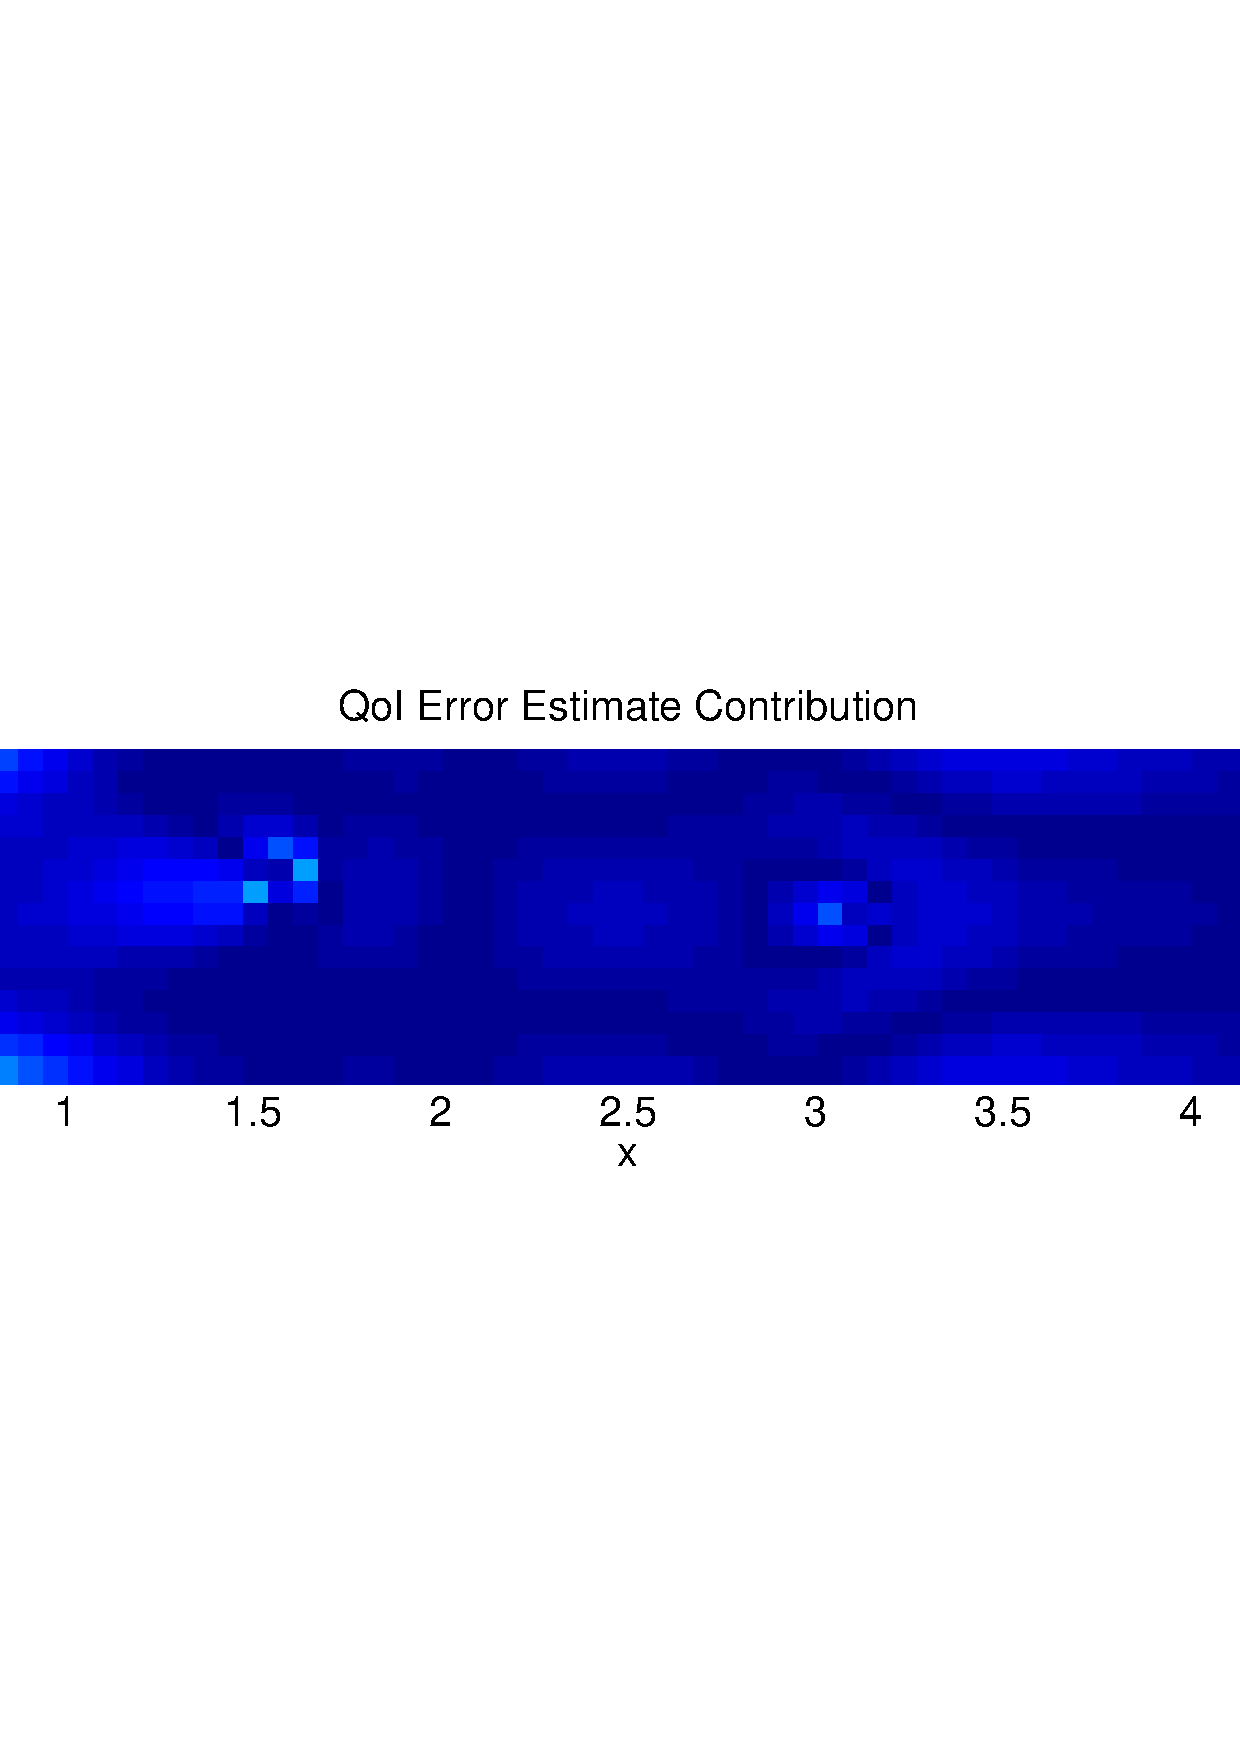
\includegraphics[width=0.51\textwidth]{svf/err_breakdown_MF03.png}
%  \vspace{-0.7\baselineskip}
%  \caption{MF$_3$ ($30\%$ HF)}
%  \vspace{0.8\baselineskip}
%\end{subfigure}
%\begin{subfigure}[b]{\textwidth}
%	\centering
%	\includegraphics[width=0.48\textwidth]{svf/cd_cdr_MF04_divvy.png}
%  \includegraphics[width=0.51\textwidth]{svf/err_breakdown_MF04.png}
%  \vspace{-0.7\baselineskip}
%  \caption{MF$_4$ ($40\%$ HF)}
%  \vspace{0.8\baselineskip}
%\end{subfigure}
%\begin{subfigure}[b]{\textwidth}
%	\centering
%	\includegraphics[width=0.48\textwidth]{svf/cd_cdr_MF05_divvy.png}
%  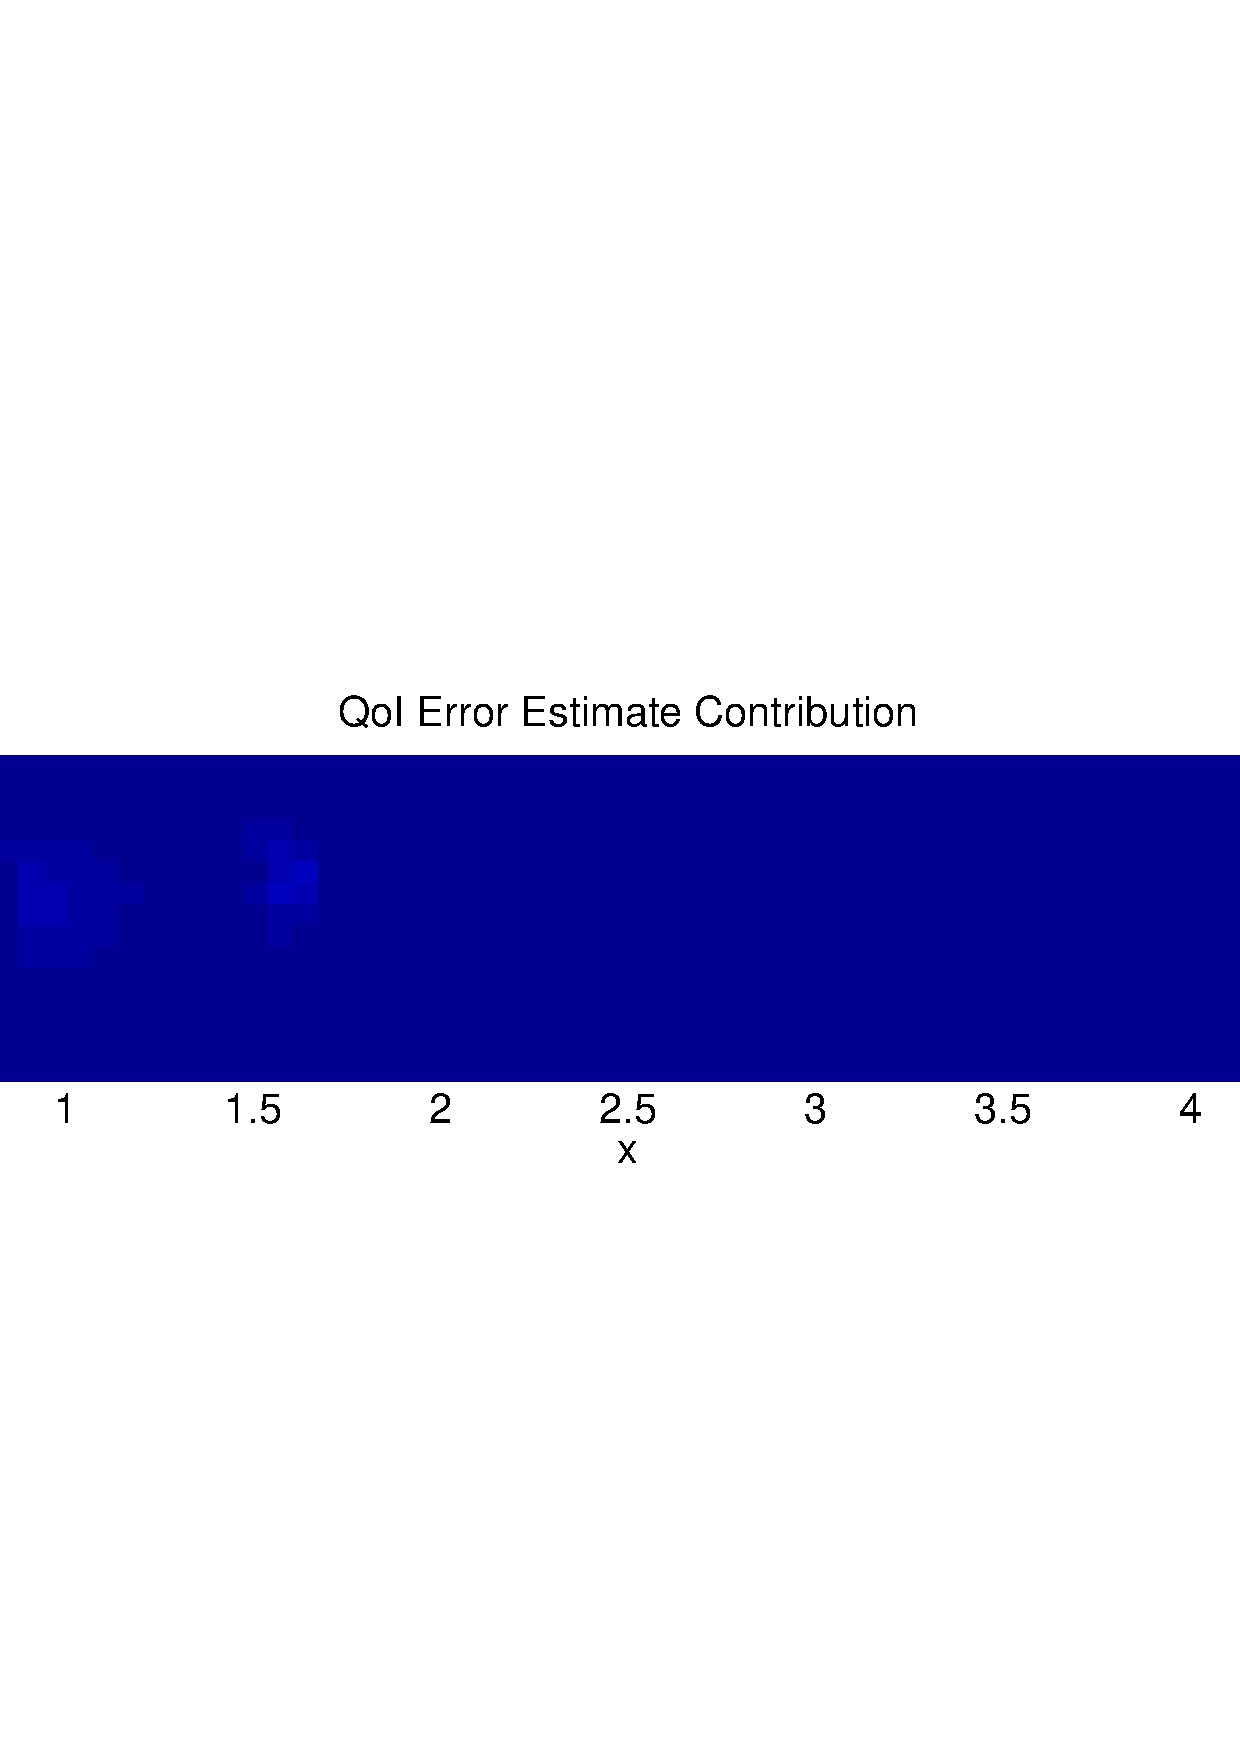
\includegraphics[width=0.51\textwidth]{svf/err_breakdown_MF05.png}
%  \vspace{-0.7\baselineskip}
%  \caption{MF$_5$ ($50\%$ HF)}
%  \vspace{0.8\baselineskip}
%\end{subfigure}
\subfloat[MF$_6$ ($60\%$ HF)]{
	\includegraphics[width=0.46\textwidth]{svf/cd_cdr_MF06_divvy.png}
  \includegraphics[width=0.49\textwidth]{svf/err_breakdown_MF06.png}
}
\caption{Local error contributions (right) and domain division (left; low-fidelity constant-parameter model used in red portion, high-fidelity field-parameter model used in blue portion) for mixed-fidelity models. The (weighted) residual, and thus the local error contribution, tends to spike sharply at the interface between the low- and high-fidelity regions; the color range is truncated to make the error distribution visible elsewhere in the domain.}
\label{fig:svfRef}
\end{figure}
%
Comparing to \cref{fig:baseRef}, we see that in this case the local error contribution is not as greatly concentrated around the QoI region and the nearest data point; here, all three data points and the QoI region have associated regions of sufficiently similar high local error that all are refined in the first iteration. This reflects the global nature of the differences between the low- and high-fidelity models; the parameter field in all the low-fidelity regions is constant and equal. 

The corresponding true and estimated absolute errors in the QoI are shown in \cref{fig:svfErr}.
%
\begin{figure}[htbp]
\centering
\includegraphics[width=0.8\textwidth]{svf/err_est.pdf}
\caption{True and estimated absolute relative error in QoI, plotted as a function of the percentage area of the domain in which the high-fidelity field-parameter model is used.}
\label{fig:svfErr}
\end{figure}
%
In this case, we see that we must use the high-fidelity model in most of the domain in order to get an accurate QoI. The adaptive algorithm requires us to use the field representation of the high-fidelity model in much of the left half of the domain; this reflects the topology of the inferred parameter field in the high-fidelity inverse problem, which is only relatively constant towards the right portion of the domain. We also see that in this case, compared to the example in \cref{sec:cdvcdrBaseRef}, increasing the proportion of the domain in which the high-fidelity model is used does not monotonically decrease the error in the QoI. 
%\if{0} %--*--*--*--*--*--*--*--*--*--*--*--*--*--*--*--*--*--*--*--*--*--*--*--*--*--*--*--*--*--*--
%------------------------------------------------------------------------------------------------------------------------%
\subsection{Convection-Diffusion(-Highly Nonlinear Reaction)}
%------------------------------------------------------------------------------------------------------------------------%
\red{Not sure should even keep this section...if we split the supplementary adjoint solve, then the condition for adaptivity being more efficient doesn't depend on the linear solver...we don't need this section to make a cost argument if we have the 3D example...having this section seems to be overkill/redundant if all we want to say is that 'sometimes we need continuation for the HF inverse problem'...if we want to make a 'robustness' argument, then merge with whatever vikram writes about operator continuation interpretation?

Can't seem to replicate this...in HF continuation code, going up to 1000 with steps of 100 is fine, with both gmres and superlu...perhaps there was a bug/copy-paste mistake in the manual continuation version? All notes on this run were accidentally lost, so...
%------------------------------------------------------------%
\subsubsection{Results}
%------------------------------------------------------------%

We consider the convection-diffusion-reaction term described in \cref{sec:cdvcdr}, with a reaction term $k_r=-616$ in the high-fidelity model. This reaction term is large enough that the Newton solver will not converge with a zero initial guess. We first solve the inverse problem with the low-fidelity model ($k_r=0$), and then use a simple continuation approach, using the solution at one value of $k_r$ as the initial guess for the next.\footnote{not arclength continuation, which is more difficult to implement, though libMesh appears to have a class for such continuation, which we can use if this seems like a viable direction} We increase the reaction term in increments of $\Delta k_r=100$, and halve the increment each time the step is too large (Newton solver does not converge at the next $k_r$ value). From $k_r=0$ to $k_r=-616$, this results in 9 continuation steps being taken.

%------------------------------------------------------------%
\subsubsection{Computational Complexity}
%------------------------------------------------------------%

We compare the complexity of\cref{alg:refSeries} and the continuation method for the high fidelity problem, in the context of the analysis developed in \cref{sect:alg_complexity}. For the high fidelity problem, with  with 9 continuation steps, we have $\sum\limits_{i=1}^{C} K_i=30$. 
 
With Gaussian elimination chosen as the linear solver, this gives us $T < 3$, i.e.\ a budget of 2 adaptive steps. Using \cref{alg:refSeries} with 2 refinement steps, and only $10\%$ of the domain refined to use the high-fidelity model, the estimated relative error is $<1\%$. Indeed, the ratio $\frac{C_{MF}}{C_{HF}}$ was $\frac{24}{30}$, indicating about $20\%$ reduction in computational cost, with the worst case linear solver used. 

In other words, on using \cref{alg:refSeries} for a highly nonlinear problem, even with the worst case linear solver, one can get to $<1\%$ error in the QoI, with a $20\%$ reduction in computational cost, while avoiding any need for continuation to handle nonlinearities. }
\fi{0} %--*--*--*--*--*--*--*--*--*--*--*--*--*--*--*--*--*--*--*--*--*--*--*--*--*--*--*--*--*--*--

%------------------------------------------------------------------------------------------------------------------------%
\subsection{Convection-Diffusion(-Reaction) in 3D} \label{sec:cdvcdr3D}
%------------------------------------------------------------------------------------------------------------------------%

\red{In the previous examples, although the low- and high-fidelity models are sufficiently different to illustrate the behavior of \cref{alg:refSeries}, they are both simple enough and similar enough that using \cref{alg:refSeries} saves little, if any, time. In this section, we consider a more realistic pair of models which differ in the physics included, and demonstrate computational savings when using the adaptive algorithm, while still achieving a small error in the QoI. In \cref{sec:setup3D} we describe the setup of the models and their inverse problems, and in \cref{sec:ref3D} we describe the results of applying \cref{alg:refSeries} to this pair of models.}

%------------------------------------------------------------%
\subsubsection{Problem Setup} \label{sec:setup3D}
%------------------------------------------------------------%

The two models share a box domain $\Omega(x_1,x_2,x_3)$ which is $2300$m, $1650$m, and $100$m long in the $x_1$, $x_2$, and $x_3$ directions, respectively. We will refer to the positive and negative directions in $x_1$ as ``east" and ``west", respectively. The high-fidelity model is a single-species convection-diffusion-reaction equation with a nonlinear reaction term, described by
%
\begin{subequations}
\label{eq:cdvcdrHF3D}
\begin{align}
\nabla\cdot(n\vec{V}u - nD\nabla u) + k_ru^2 = f(q) \quad &\text{in } \Omega, \label{eq:HFeq3D}\\
u = 5 \quad &\text{on } \partial \Omega_{west}, \\
\frac{\partial u}{\partial n} = 0 \quad &\text{on }\partial\Omega_{east}, \\
\hat{n}\cdot(n\vec{V}u - nD\nabla u) = 0 \quad &\text{on }\partial\Omega\backslash(\partial\Omega_{east}\cup\partial\Omega_{west}),
\end{align} 
\end{subequations}
%
where the state $u$ is the mass-fraction (in parts-per-billion) of some contaminant species and $f(q)$ is a source/sink field. The velocity field is a constant $\vec{V}=(2.1,0,0)$ m/day. Given this velocity field and letting the molecular diffusion be negligble, we follow \cite{Vestedetal93} to express the (diagonal) dispersion tensor $D$ as $D_{11}=\alpha_{LH}V_1$, $D_{22}=\alpha_{TH}V_1$, and $D_{33}=\alpha_{TV}V_1$, where $\alpha_{LH}=100$m, $\alpha_{TH}=40$m, and $\alpha_{TV}=4$m are the longitudinal horizontal, transverse horizontal, and transverse vertical dispersivities, respectively; the dispersivity values were drawn from within the range of observed values in various porous media \cite{Davis86}. We have porosity $n=0.1$. The reaction coefficient is $k_r=4.2\cdot10^{-4}$ 1/day, chosen from within the wide range of reaction-rate coefficients for second-order reactions. Although the reaction term $k_ru^2$ does not correspond to any particular reaction of any particular species, we note that, in addition to second-order elementary reactions, a quadratic reaction term can appear in models of dissolution/precipitation processes in porous media \cite{Aha97} and biochemical degredation of petroleum hydrocarbons in soils \cite{Jack94}.

The low-fidelity model,
%
\begin{equation}
\nabla\cdot(n\vec{V}u - nk_d\nabla u) = f(q) \quad \text{in } \Omega, \label{eq:LFeq3D}
\end{equation}
%
differs in the removal of both the reaction term and the anisotropy of the dispersion tensor; the dispersion tensor $D$ is replaced with a scalar $k_d=D_{11}$. The boundary conditions remain unchanged. As in the previous examples in \cref{sec:cdvcdr}, the mixed-fidelity models are formed by dividing the domain into complementary subdomains $\Omega_{HF}$ and $\Omega_{LF}$, where \cref{eq:HFeq3D,eq:LFeq3D} are solved, respectively. The QoI we wish to calculate is again an integral of the state over a region $\Omega_I$. 

The unknown parameters we wish to infer correspond to the source term $f(q)=q$; we impose $f(q)=q=0$ on the boundary $\partial\Omega$. Observations at 18 points in the domain are artificially generated by running the high-fidelity model on a finer mesh. The locations of the observations as well as the QoI region $\Omega_I$ are shown in \cref{fig:setup3D}. We use a regularization term $\frac{\beta}{2}\int_\Omega \|\nabla f(q)\|_2^2\:\textrm{d}V$.
%
\begin{figure}[htbp]
\centering
\includegraphics[width=0.4\textwidth]{series3D/setup_aerial_nolegend.pdf} \hfill
\includegraphics[width=0.55\textwidth]{series3D/setup_3view.pdf} \\ 
\vspace{\baselineskip}
\includegraphics[width=0.6\textwidth]{series3D/setup_side_view.pdf}
\caption{Three views of the locations of the observations and the QoI region.}
\label{fig:setup3D}
\end{figure}
%
We continue to use the FEM with a continuous Galerkin formulation and Lagrange elements. The domain is discretized by a regular mesh of hexahedrons, with 25, 45, and 30 elements along the $x_1$, $x_2$, and $x_3$ directions, respectively; each variable has 37,076 degrees of freedom. The cell P\'{e}clet number is less than one and so no stabilization is used.

%------------------------------------------------------------%
\subsubsection{Adaptive Model Refinement Results} \label{sec:ref3D}
%------------------------------------------------------------%

We now present the results of solving the inference problem using \cref{alg:refSeries}, with a relative error tolerance of $1\%$. At each iteration, we choose the $5\%$ of the basis functions with the largest error for model refinement; since each linear Lagrange basis function has eight elements in its support, the number of additional elements marked for refinement in each iteration may be greater. All simulations are run on a single processor; we use the default nonlinear solver in \texttt{libMesh} (Newton's method with Brent line-search), and linear solves are performed using PETSC's GMRES solver, preconditioned by incomplete factorization. \Cref{tab:ref3D} shows the runtime and error at the end of each adaptive iteration. The high-fidelity inverse problem is solved by using natural continuation on the reaction parameter to avoid stalling the Newton iterations; only two steps are required: $k_r=0$, then $k_r=4.2\cdot10^{-4}$. Each iteration of the adaptive algorithm uses the solution of the previous iteration as its initial guess. 
%
\begin{table}[htbp]
\caption{Runtime and relative errors of adaptive algorithm iterations given relative error tolerance of $1\%$; relative errors are given with respect to the true high-fidelity QoI.}
\label{tab:ref3D}
\centering
\begin{tabular}{|c|c|c|c|c|c|c|c|}
\hline
\multirow{2}{*}{Case} & \multirow{2}{*}{$\%$HF} & \multirow{2}{*}{QoI} & Error & Error & $\%$ Relative & Iteration \\ 
& & & (Estimated) & (Actual) & Error (Actual) & Time (s) \\ \hline
LF   & 0    & 133730 & -4024 & -6020 & -4.71 & 622 \\
MF01 & 10.0 & 125073 & 4404  & 2637  & 2.06  & 419 \\
MF02 & 17.7 & 123093 & 6761  & 4617  & 3.62  & 378 \\
MF03 & 25.0 & 123460 & 6354  & 4250  & 3.33  & 369 \\
MF04 & 32.9 & 125291 & 2242  & 2419  & 1.89  & 454 \\
MF05 & 39.7 & 126314 & 2445  & 1396  & 1.09  & 324 \\
MF06 & 47.2 & 126927 & 1070  & 783   & 0.61  & 348 \\
HF   & 100  & 127710 & --    & --     & --   & 427 \\ \hline
\end{tabular}
\end{table}
%

Compared to the previous examples in \cref{sec:cdvcdr} with similar physics in the pair of models, we observe that the error in the QoI (both true and estimated) does not decrease monotonically as the percentage of the domain in which the high-fidelity model is used increases. We also observe that any oscillations tend to occur within the first few iterations; continuing the adaptive algorithm beyond those iterations shown in \cref{tab:ref3D} monotonically decreases the QoI errors with increased refinement, until the high-fidelity model is used in the entire domain.

The domain divisions for the six adaptive iterations are shown in \cref{fig:divvy3D}. We see that the error decomposition causes the first refinement iteration to target the QoI region and observations; similarly to the behavior seen in \cref{sec:cdvcdrBaseRef}, those measurement points furthest downstream of the QoI region are refined later. Around the QoI region, the first iteration refines the domain completely in the $x_3$ direction, possibly reflecting the large difference in the high-fidelity dispersion tensor $D$ and the low-fidelity dispersion coefficient in the $x_3$ direction.
%
\begin{figure}[htbp]
\centering
\subfloat[MF$_1$]{
\includegraphics[width=0.31\textwidth]{series3D/run_invcrime/divvy1_whitebg_puff.png} 
}
\subfloat[MF$_2$]{
\includegraphics[width=0.31\textwidth]{series3D/run_invcrime/divvy2_whitebg_puff.png} 
}
\subfloat[MF$_3$]{
\includegraphics[width=0.31\textwidth]{series3D/run_invcrime/divvy3_whitebg_puff.png} 
} \\
\subfloat[MF$_4$]{
\includegraphics[width=0.31\textwidth]{series3D/run_invcrime/divvy4_whitebg_puff.png} 
}
\subfloat[MF$_5$]{
\includegraphics[width=0.31\textwidth]{series3D/run_invcrime/divvy5_whitebg_puff.png} 
}
\subfloat[MF$_6$]{
\includegraphics[width=0.31\textwidth]{series3D/run_invcrime/divvy6_whitebg_puff.png} 
}
\caption{Domain division for mixed-fidelity models: low-fidelity convection-diffusion model used in red portion, high-fidelity convection-diffusion-reaction model used in blue portion (intermediate colors due to transparency indicate a mix of the two models along the line of sight); $x_3$ direction scaled for clarity.}
\label{fig:divvy3D}
\end{figure} 
%

In this case, the high-fidelity inverse problem is only mildly nonlinear and requires few continuation steps and Newton iterations to converge; there are no savings in computational time from using the adaptive algorithm instead of solving the high-fidelity inverse problem. However, one would expect solving the high-fidelity inverse problem to require more time relative to using the adaptive algorithm as the nonlinearity of the high-fidelity model increases. 

\Cref{alg:refSeries} is also ammenable to an offline-online decomposition, analagous to that proposed in \cite{LiebWill13}. The offline phase would consist of adaptively creating a mixed-fidelity model with an appropriate error tolerance given some expected observations $d^*$. When new data is received, one can then solve the inverse problem with the chosen mixed-fidelity model and the new data, and, if desired, compute an error estimate for the QoI. The mixed-fidelity inverse problems can be expected to require less time to solve than the high-fidelity inverse problems.

To illustrate the offline-online application, we generate ten sets of noisy observations to represent the new data gained during the online phase; the noisy observations are generated by taking the observations used in the adaptive algorithm and adding Gaussian white noise with standard deviation of $\sigma=0.05$ (equivalent to anywhere from $1.7\%$ to $17\%$ of the observed values). We then solve the inverse problem using each of the mixed-fidelity models depicted in \cref{tab:ref3D,fig:divvy3D} as well as the high-fidelity model. The high-fidelity inverse problem is solved using the same two continuation steps; the first continuation step is also used as an initial guess for the mixed-fidelity inverse problems. The auxiliary and supplementary adjoint variables simply have a zero initial guess. \Cref{tab:ref3D_newdata_QoI,tab:ref3D_newdata_times} shows the average QoI values and error estimates and solution times over the ten datasets.
%
\begin{table}
\caption{Average QoI values and errors from solving inverse problem with mixed- and high-fidelity models and noisy data; relative errors are with respect to true high-fidelity QoI.}
\label{tab:ref3D_newdata_QoI}
\centering
\begin{tabular}{|c|c|c|c|c|c|}
\hline
\multirow{2}{*}{Case} & \multirow{2}{*}{$\%$HF} & \multirow{2}{*}{QoI} & Error & Error & $\%$ Relative  \\ 
& & & (Estimated) & (Actual) & Error (Actual) \\ \hline
MF01 & 10.0 & 123672 & 4328 & 2599 & 2.08  \\
MF02 & 17.7 & 122073 & 6331 & 4197 & 3.34  \\
MF03 & 25.0 & 122409 & 5972 & 3861 & 3.06  \\
MF04 & 32.9 & 124011 & 3449 & 2260 & 1.79  \\
MF05 & 39.7 & 124852 & 2481 & 1418 & 1.12  \\
MF06 & 47.2 & 125440 & 1123 & 830  & 0.66  \\ 
HF   & 100  & 126270 & --   & --   & --     \\ \hline
\end{tabular}
\end{table}
%
\begin{table}
\caption{Average times to solve inverse problem and obtain error estimate with mixed- and high-fidelity models and noisy data.}
\label{tab:ref3D_newdata_times}
\centering
\begin{tabular}{ccc|c|c|c}
\cline{4-5} 
 & & & \multicolumn{2}{|c|}{Error Estimation} & \\
\cline{1-6}
\multicolumn{1}{|c|}{\multirow{3}{*}{Case}} & \multicolumn{1}{|c|}{\multirow{3}{*}{$\%$HF}} & Inverse & Auxiliary & Supplementary & \multicolumn{1}{|c|}{Total} \\
\multicolumn{1}{|c|}{} & \multicolumn{1}{|c|}{} & Problem & Variables & Adjoint & \multicolumn{1}{|c|}{Solution}\\
\multicolumn{1}{|c|}{} & \multicolumn{1}{|c|}{} & Time (s) &  Time (s) & Time (s) & \multicolumn{1}{|c|}{Time (s)}\\
\cline{1-6}
\multicolumn{1}{|c|}{MF01}  & \multicolumn{1}{|c|}{10.0}  & 173 & 48 & 103 & \multicolumn{1}{|c|}{323} \\ \hline
\multicolumn{1}{|c|}{MF02}  & \multicolumn{1}{|c|}{17.7}  & 191 & 49 & 104 & \multicolumn{1}{|c|}{343} \\ \hline
\multicolumn{1}{|c|}{MF03}  & \multicolumn{1}{|c|}{25.0}  & 192 & 51 & 109 & \multicolumn{1}{|c|}{352} \\ \hline
\multicolumn{1}{|c|}{MF04}  & \multicolumn{1}{|c|}{32.9}  & 190 & 49 & 96  & \multicolumn{1}{|c|}{334} \\ \hline
\multicolumn{1}{|c|}{MF05}  & \multicolumn{1}{|c|}{39.7}  & 188 & 49 & 92  & \multicolumn{1}{|c|}{329} \\ \hline
\multicolumn{1}{|c|}{MF06}  & \multicolumn{1}{|c|}{47.2}  & 189 & 50 & 89  & \multicolumn{1}{|c|}{327} \\ \hline
\multicolumn{1}{|c|}{HF}    & \multicolumn{1}{|c|}{100}   & 214 & -- & --  & \multicolumn{1}{|c|}{214} \\ \hline
\end{tabular}
\end{table}
%

We see that in this case, when the mixed-fidelity models are used to infer from observations different from those they were generated with, they continue to give similar relative accuracy in their QoI. We also note that the mixed-fidelity inverse problems consistently take less time to solve than the high-fidelity inverse problems; however, the high-fidelity inverse problem is still only mildly nonlinear and requires few nonlinear steps to converge, so the difference in their solution times is not large enough to justify estimating the mixed-fidelity QoI errors as well.

%------------------------------------------------------------------------------------------------------------------------%
\subsection{Combining Meshes and Physics} \label{sec:diffvcdr3D}
%------------------------------------------------------------------------------------------------------------------------%

Here we consider two models which differ in both their mesh resolution and the physics included. 

%------------------------------------------------------------%
\subsubsection{Problem Setup}
%------------------------------------------------------------%

The high-fidelity model remains the same as that described in \cref{sec:setup3D}, with the exception of the boundary condition $u=0$ on $\partial\Omega_{west}$. The low-fidelity model shares the domain and boundary condition of the high-fidelity model, but again lacks a reaction term and has a scalar dispersion coefficient; the low-fidelity model also lacks a convection term. The lack of a convection term allows the low-fidelity model to be solved on a coarser mesh. For the high-fidelity model, the domain is descretized by 32, 64, and 32 elements along the $x_1$, $x_2$, and $x_3$ directions, respectively; for the low-fidelity model, the domain is descretized by 16, 32, and 16 elements along the $x_1$, $x_2$, and $x_3$ directions, respectively. The regularization term, QoI region, and measurements remain the same as described in \cref{sec:setup3D}.

%------------------------------------------------------------%
\subsubsection{Adaptive Model Refinement Results} \label{sec:ref3D_diffmesh}
%------------------------------------------------------------%

We now present the results of solving the inference problem using \cref{alg:refSeries}, with a relative error tolerance of $0.1\%$. At each iteration, we choose the $2\%$ of the basis functions with the largest error for model refinement; again, since each linear Lagrange basis function has eight elements in its support, the number of additional elements marked for refinement in each iteration is usually greater. \Cref{tab:ref3D_diffmesh} shows the runtime and true and estimated QoI errors for each adaptive iteration; the high-fidelity inverse problem is solved in the same way as described in \cref{sec:ref3D}. The number of degrees of freedom of each of the primary (and, if applicable, auxiliary) variables at each iteration is also given; the supplementary adjoint is solved on the high-fidelity mesh and thus each of its variables has the same number of degrees of freedom as each of the primary variables in the high-fidelity inverse problem.
%
\begin{table}[htbp]
\caption{Runtime and relative errors of adaptive algorithm iterations given relative error tolerance of $0.1\%$; relative errors are given with respect to the true high-fidelity QoI.}
\label{tab:ref3D_diffmesh}
\centering
\begin{tabular}{|c|c|c|c|c|c|c|c|}
\hline
\multirow{2}{*}{Case} & \multirow{2}{*}{DOFs} & \multirow{2}{*}{QoI} & Error & Error & $\%$ Relative & Iteration \\ 
& & & (Estimated) & (Actual) & Error (Actual) & Time (s) \\ \hline
LF   & 9537  & 168710 & -16463 & -85663 & -103   & 1023 \\
MF01 & 13417 & 167366 & -7207  & -84319 & -102   & 814 \\
MF02 & 17895 & 89777  & -6208  & -6730  & -8.10  & 858 \\
MF03 & 21001 & 85880  & -2473  & -2833  & -3.41  & 922 \\
MF04 & 24528 & 83902  & -711   & -855   & -1.03  & 973 \\
MF05 & 27984 & 83119  & 32     & -72    & -0.087 & 1187 \\
HF   & 70785 & 83047  & --    & --     & --   & 457 \\ \hline
\end{tabular}
\end{table}
%
We notice that, compared to the results in \cref{sec:ref3D}, the error estimates for the low-fidelity and first mixed-fidelity models are very far from the true errors. This can be attributed to the linearization about $\Psi_{LF}$ and $\Psi_{MF_{1}}$ instead of $\Psi_{HF}$ in solving the supplementary adjoints; the large differences in the QoI for the LF and MF01 models compared to the high-fidelity QoI indicate that $\Psi_{LF}$ and $\Psi_{MF_{1}}$ are very different from $\Psi_{HF}$. This suggests that one should use more than just the error estimate to decide when to stop the adaptive algorithm; a possible additional criterion could be to require that the predicted high-fidelity QoI $I(q_{MF},u_{MF})+\epsilon_i$ for two consecutive iterations agree to within some tolerance.

The domain divisions for the five adaptive iterations are shown in \cref{fig:divvy3D_diffmesh}. We note some similarities with the series of mixed-fidelity models in \cref{fig:divvy3D}, namely that in both, the QoI region has been refined after $10\%$ refinement, and those measurement points furthest downstream of the QoI are the last to be refined around. We also see that the domain is refined completely in the $x_3$ direction first around the QoI region, again possibly reflecting the large difference in the high-fidelity dispersion tensor $D$ and the low-fidelity dispersion coefficient in the $x_3$ direction.
%
\begin{figure}[htbp]
\centering
\subfloat[MF$_1$ ($5.2\%$ HF)]{
\includegraphics[width=0.31\textwidth]{series3D/run_diff_mesh/divvy1_whitebg_puff.png} 
}
\subfloat[MF$_2$ ($11.4\%$ HF)]{
\includegraphics[width=0.31\textwidth]{series3D/run_diff_mesh/divvy2_whitebg_puff.png} 
}
\subfloat[MF$_3$ ($16.3\%$ HF)]{
\includegraphics[width=0.31\textwidth]{series3D/run_diff_mesh/divvy3_whitebg_puff.png} 
} \\
\subfloat[MF$_4$ ($22.0\%$ HF)]{
\includegraphics[width=0.31\textwidth]{series3D/run_diff_mesh/divvy4_whitebg_puff.png} 
}
\subfloat[MF$_5$ ($27.7\%$ HF)]{
\includegraphics[width=0.31\textwidth]{series3D/run_diff_mesh/divvy5_whitebg_puff.png} 
}
\caption{Domain division for mixed-fidelity models: low-fidelity convection-diffusion model used in red portion, high-fidelity convection-diffusion-reaction model used in blue portion (intermediate colors due to transparency indicate a mix of the two models along the line of sight); $x_3$ direction scaled for clarity.}
\label{fig:divvy3D_diffmesh}
\end{figure} 
%
We notice in \cref{tab:ref3D_diffmesh} that although the mixed-fidelity models have fewer degrees of freedom than the high-fidelity model, it is still faster to solve the high-fidelity inverse problem than to solve a mixed-fidelity inverse problem and obtain an error estimate. This can be attributed to the extra time needed to construct systems and project solutions when seeking an error estimate, as well as the mild nonlinearity of the high-fidelity problem and solving for the supplementary adjoint on the high-fidelity mesh. For larger problems, it is expected that the computational costs will be dominated by the linear solves. For comparison, we select one of the sets of noisy observations described in \cref{sec:ref3D} and solve the inverse problem using each of the mixed-fidelity models depicted in \cref{tab:ref3D_diffmesh,fig:divvy3D_diffmesh} as well as the high-fidelity model. The low-fidelity inverse problem is first solved and used as an initial guess for the higher-fidelity problems; we note that although there is a linear model that is more similar to the high-fidelity model than the low-fidelity model (i.e., convection-diffusion with anisotropic diffusivity on the high-fidelity mesh) and thus would serve as a better initial guess, its existence is specific to our particular choice of models. \Cref{tab:ref3D_newdata_QoI_diffmesh,tab:ref3D_newdata_times_diffmesh} shows the QoI values and error estimates and solution times for the (non)linear solves, not including the time needed to obtain the initial guess.
%
\begin{table}
\caption{QoI values and errors from solving inverse problem with mixed- and high-fidelity models and noisy dataset; relative errors are with respect to true high-fidelity QoI.}
\label{tab:ref3D_newdata_QoI_diffmesh}
\centering
\begin{tabular}{|c|c|c|c|c|c|}
\hline
\multirow{2}{*}{Case} & \multirow{2}{*}{DOFs} & \multirow{2}{*}{QoI} & Error & Error & $\%$ Relative  \\ 
& & & (Estimated) & (Actual) & Error (Actual) \\ \hline
MF01 & 13417 & 153999 & 2786500 & -74228 & -93.05  \\
MF02 & 17895 & 85705  & -6496   & -5934  & -7.44  \\
MF03 & 21001 & 82544  & -3721   & -2773  & -3.48  \\
MF04 & 24528 & 80684  & -2139   & -913   & -1.14  \\
MF05 & 27984 & 80154  & -1688   & -383   & -0.48 \\
HF   & 70785 & 79771  & -- & -- &   \\ \hline
\end{tabular}
\end{table}
%
\begin{table}
\caption{Times to solve inverse problem and obtain error estimate with mixed- and high-fidelity models and noisy dataset.}
\label{tab:ref3D_newdata_times_diffmesh}
\centering
\begin{tabular}{ccc|c|c|c}
\cline{4-5} 
 & & & \multicolumn{2}{|c|}{Error Estimation} & \\
\cline{1-6}
\multicolumn{1}{|c|}{\multirow{3}{*}{Case}} & \multicolumn{1}{|c|}{\multirow{3}{*}{DOFs}} & Inverse & Auxiliary & Supplementary & \multicolumn{1}{|c|}{Total} \\
\multicolumn{1}{|c|}{} & \multicolumn{1}{|c|}{} & Problem & Variables & Adjoint & \multicolumn{1}{|c|}{Solution}\\
\multicolumn{1}{|c|}{} & \multicolumn{1}{|c|}{} & Time (s) &  Time (s) & Time (s) & \multicolumn{1}{|c|}{Time (s)}\\
\cline{1-6}
\multicolumn{1}{|c|}{MF01}  & \multicolumn{1}{|c|}{13147}  & 132  & 141 & 785 & \multicolumn{1}{|c|}{1058} \\ \hline
\multicolumn{1}{|c|}{MF02}  & \multicolumn{1}{|c|}{17895}  & 209  & 172 & 177 & \multicolumn{1}{|c|}{558} \\ \hline
\multicolumn{1}{|c|}{MF03}  & \multicolumn{1}{|c|}{21001}  & 312  & 169 & 188 & \multicolumn{1}{|c|}{669} \\ \hline
\multicolumn{1}{|c|}{MF04}  & \multicolumn{1}{|c|}{24528}  & 275  & 177 & 184 & \multicolumn{1}{|c|}{636} \\ \hline
\multicolumn{1}{|c|}{MF05}  & \multicolumn{1}{|c|}{27984}  & 403  & 283 & 189 & \multicolumn{1}{|c|}{875} \\ \hline
\multicolumn{1}{|c|}{HF}    & \multicolumn{1}{|c|}{70785}  & 2364 & --  & --  & \multicolumn{1}{|c|}{2364} \\ \hline
\end{tabular}
\end{table}
%



\section{Conclusion}\label{sect:conc}


\appendix
%\chapter{Notation} \label{appendix}

For quick reference, the following table summarizes notation used throughout this thesis 
(in alphabetical order).

\begin{table}[!ht]
\caption{Summary of Notation}
\begin{center}
\begin{tabular}{c|l}
\textbf{Symbol} & \textbf{Meaning} \\
\hline \hline
$q$  &   Model parameters \\
$u$  &   Model state\\
\end{tabular}
\end{center}
\end{table}

\include{biblio}
\end{document}
